\documentclass{standalone}
\usepackage{tikz}
\usetikzlibrary{shapes}
\usepackage{amsmath}


\tikzstyle{startstop} = [rectangle, rounded corners, text width=2cm,text centered, minimum height=1cm, draw=black]
\tikzstyle{io} = [trapezium, trapezium left angle=70,trapezium right angle=110, text width=3.3cm, minimum height=1cm, text centered, draw=black, trapezium stretches=true]
\tikzstyle{process} = [rectangle, text width=3.3cm, minimum height=1cm, text centered, draw=black]

\begin{document}
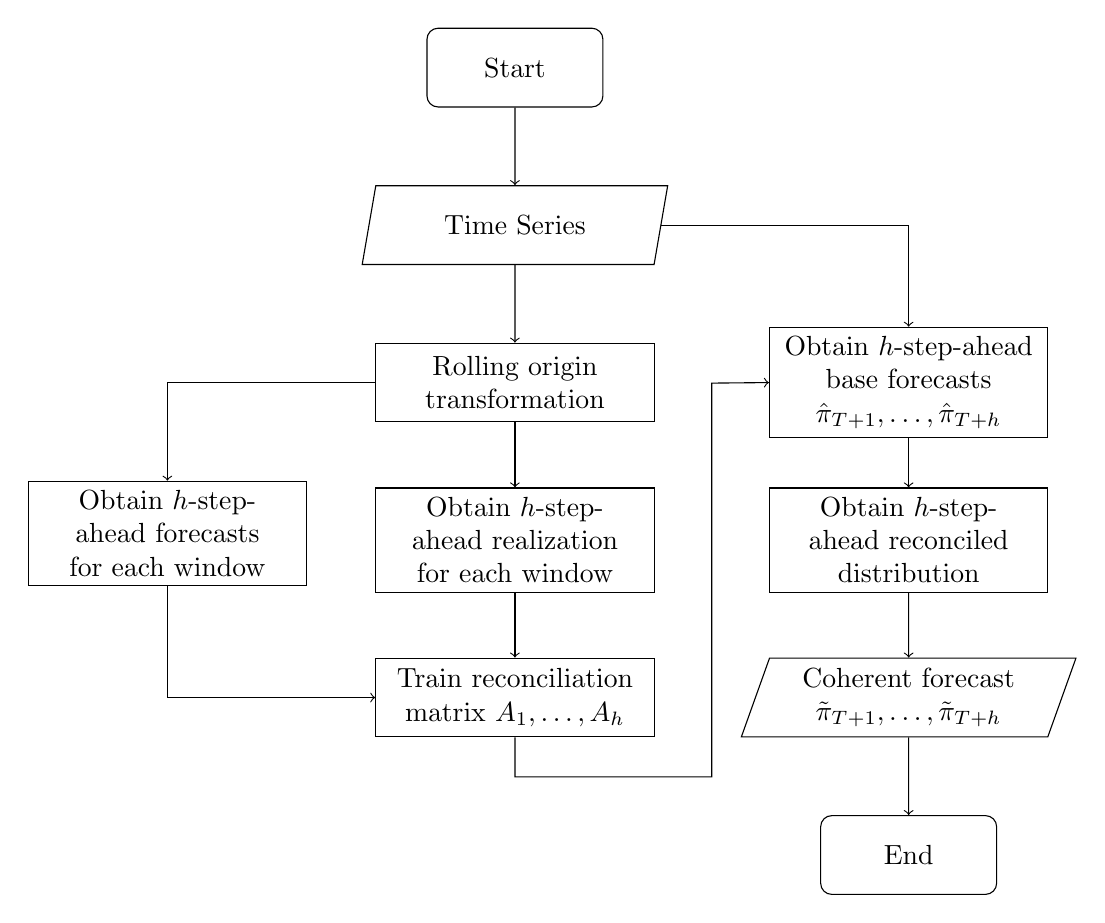
\begin{tikzpicture}[node distance=2cm]
    
    \node(start)[startstop]{Start};
    \node(in)[io, below of=start]{Time Series};

    \node(rollingorigin)[process, below of=in]{Rolling origin transformation};

    \node(train1)[process, below left of=rollingorigin, xshift=-3cm, yshift=-0.5cm]{Obtain $h$-step-ahead forecasts for each window};
    \node(train2)[process, below of=rollingorigin]{Obtain $h$-step-ahead realization for each window};

    \node(train3)[process, below of=train2]{Train reconciliation matrix $A_1,\dots,A_h$};

    \node(forecast1)[process,right of=rollingorigin, xshift=3cm]{Obtain $h$-step-ahead base forecasts $\hat{\mathbf{\pi}}_{T+1},\dots,\hat{\mathbf{\pi}}_{T+h}$};
    \node(forecast2)[process, below of=forecast1]{Obtain $h$-step-ahead reconciled distribution};
    \node(output)[io, below of=forecast2]{Coherent forecast $\tilde{\mathbf{\pi}}_{T+1},\dots,\tilde{\mathbf{\pi}}_{T+h}$};
    \node(end)[startstop, below of=output]{End};

    \draw[->] (start) edge (in) 
        (in) edge (rollingorigin) ;
    \draw[->] (rollingorigin) -| (train1) ;
    \draw[->] (rollingorigin.south) -| (train2) ;

    \draw[->] (train1) |- (train3);
    \draw[->] (train2.south) -| (train3);
    \draw[->] (in.east) -| (forecast1.north);
    \draw[->] (train3.south) |- ++(2.5,-0.5) -- ++(0,5.0) -- (forecast1.west);
    \draw[->] (forecast1) -- (forecast2);


    \draw[->] (forecast2) -- (output);
    \draw[->] (output) -- (end);
    
\end{tikzpicture}
\end{document}
